
\documentclass{../thesis}

\subtitle{Diplomarbeit}
\title{Algorithmen zur automatisierten Generalisierung durch Zusammenfassung von Linienzügen in OpenStreetMap\\ für konkrete Spezialfälle}
\author{Arne Johannessen}
\publishers{betreut durch\\ Prof. Dr. rer. nat. Detlef Günther-Diringer\\ und\\ Dipl.-Wi.-Ing. Frederik Ramm}
%\date{Arbeitsentwurf}
%\dedication{}

%\ccbysa
% https://creativecommons.org/licenses/by-sa/4.0/legalcode.de
% https://wiki.creativecommons.org/wiki/License_Versions
% ODBL: 2009 <http://www.ifross.org/artikel/open-database-license-odbl-veroeffentlicht>

% je4
%\pdfinfo{
%  /Author (Name)
%  /Title (Titel der Diplomarbeit)
%  /Producer     (pdfeTex 3.14159-1.30.6-2.2)
%  /Keywords ()
%}
%\hypersetup{
%pdftitle=Titel der Diplomarbeit,
%pdfauthor=Name,
%pdfsubject={Diplomarbeit},
%pdfproducer={pdfeTex 3.14159-1.30.6-2.2},
%colorlinks=false,
%%pdfborder=0 0 0	% keine Box um die Links!
%}

\begin{document}

\maketitle

%\begin{abstract}
%\end{abstract}

\tableofcontents

\renewcommand{\onlyinsubfile}[1]{}
%\renewcommand{\notinsubfile}[1]{#1}
\renewcommand{\BibTeXenabled}{1}

\setcounter{chapter}{1} %% UTF-8

% single-chapter commands
\documentclass[../main/thesis.tex]{subfiles}
\begin{document}


\chapter{Einleitung \emph{[ausstehend]}}

\begin{itemize}
	\item erste, grobe Einführung ins Thema
	\item knapper Abriss des Kontextes der Fragestellung in Grundzügen (vgl. Themenblatt)
	\item was macht die Fragestellung interessant? (Motivation -- evtl. schon einzelne Anwendungsfälle umreißen)
	\item Gesamtüberblick der Arbeit einschließlich ihrer Ergebnisse, roter Faden als Orientierung für den Leser
	\item Eindruck an den Leser: warum soll er diese Arbeit weiterlesen oder welche Kapitel kann er überspringen
\end{itemize}

% auch Kontext _meiner_ Arbeit erklären -> Kooperation mit Geofabrik etc. -DGD
% Im weiteren Text der Arbeit können (und in gewissem Sinne _sollten_) Passagen aus dem Themenblatt 1:1 auftauchen, um den Bezug herzustellen. -DGD



% single-chapter commands
\end{document}

\subfile{../chapter2/Analyse}
\subfile{../chapter3/Spezifikation}
\subfile{../chapter4/Algorithmen}
\subfile{../chapter5/Implementierung}
%% UTF-8

% single-chapter commands
\documentclass[../main/thesis.tex]{subfiles}
\onlyinsubfile{\setcounter{chapter}{5}}  % single-chapter command
\begin{document}


\chapter{Ergebnisdiskussion}
% Beschreibung, was tatsächlich die Software ausspuckt, wo's hakt und wo ich noch gebastelt habe
% alles NUR im "Anwendungskontext", d.h. in Bezug auf die Ausgabe-Geodaten, nicht die Softwarequalität (das war in 5.4!)
% Schritt für Schritt Probleme sammeln und katalogisieren

Die in Kap. 4 und 5 entwickelte Software ist das Ergebnis dieser Arbeit. Hier diskutiert werden soll die Arbeitsweise dieser Software und die Qualität der von ihr ausgegebenen Geodaten in Bezug auf die Aufgabenstellung.

% möglichst auch Untersuchung der Anwendung des Algorithmus auf Straßen in unterschiedlichen Regionen der Welt



\section{Anwendung in einfachen Situationen}

Bei Anwendung der mit dieser Arbeit entwickelten Software auf Geodaten aus der \osm-Datenbank zeigt sich, dass die implementierten Algorithmen grundsätzlich funktionieren.

\onefigure{t}{
	\twofigures{H}{
		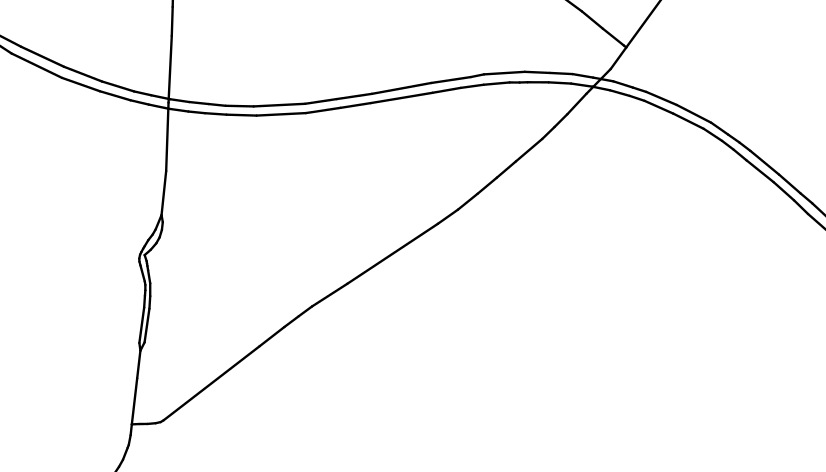
\includegraphics[width=\ScaleIfNeeded]{../chapter6/result-trivial-in}
	}{
		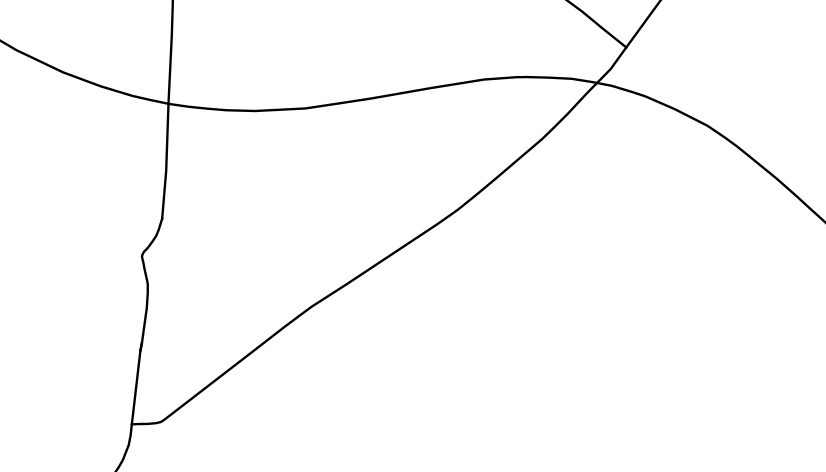
\includegraphics[width=\ScaleIfNeeded]{../chapter6/result-trivial-out}
	}
	% map extents (Google Mercator) 778753 6607040 780874 6608252; 0.2mm stroke
	\caption{Ergebnis der Software im einfachen Fall (links Eingangsdaten, rechts Generalisierungsergebnis; Autobahn L~124 bei Köln-Gremberg)}
	\label{fig:result-trivial}
}

In Abbildung~\ref{fig:result-trivial} sind links \osm-Linienzüge in der einfachen Situation einer Autobahn ohne Anschlussstellen nebst innerstädtischen Sammelstraßen zu sehen.
Durch Anwendung der Software ergibt sich das rechts dargestellte automatisiert zusammengefasste Ergebnis.
Anstelle der beiden Richtungsfahrbahnen der Autobahn gibt es nun nur noch eine gemeinsame Mittellinie.
Die Nähe zu nachgeordneten Straßen und deren planfreie Kreuzung mit der Autobahn stört die Generalisierung nicht.
Auch eine Strecke paralleler Fahrbahnen im nachgeordneten Netz wurde trotz eines scharfen Knicks erfolgreich als parallel erkannt und zusammengefasst.

Abbildung~\ref{fig:result-trivial-styled} zeigt beispielhaft, wie sich dieses Generalisierungsergebnis sinnvoll visualisieren ließe.
Die Software kennzeichnet die zusammengefassten Linienzüge als generalisiert.
Zusätzlich gibt die Software einzelne \term{tags} der \osm-Quelldaten mit aus.
Anhand dieser Attribute können leicht Regeln mit jeweils passenden Liniearsignaturen definiert werden.

\onefigure{t}{
	\twofigures{H}{
		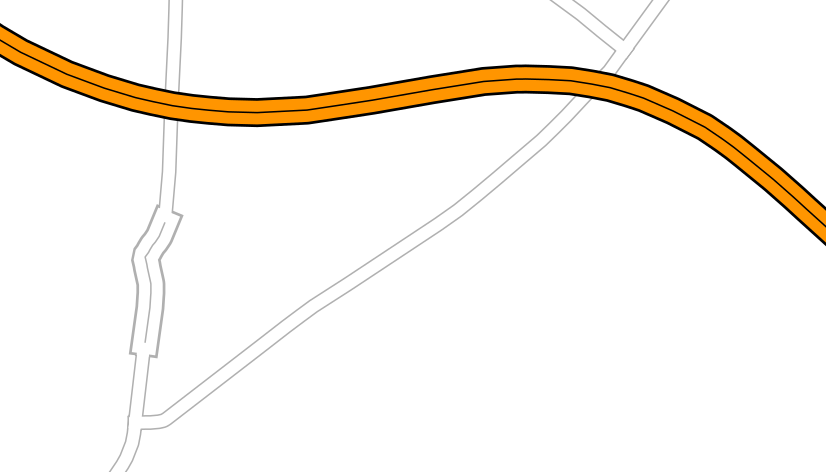
\includegraphics[width=\ScaleIfNeeded]{../chapter6/result-trivial-styled}
	}{
		\includegraphics[width=\ScaleIfNeeded]{../chapter6/result-trivial-rules}
	}
	\caption{Visualisierung des Generalisierungsergebnisses (links Kartendarstellung, rechts Screenshot der Zeichenregeln in QGIS)}
	\label{fig:result-trivial-styled}
}

\begin{itemize}
\item möglichst quantifizieren („bei Eingabedaten von xy km Autobahn gibt es z Problemsituationen“)
\item offen: Nicht-motorway/trunk sind schwieriger, da kleinere Kurvenradien. Funktioniert's hier? Wo nicht?
\item offen: Die \textproc{Distanz} zweier Straßen ist eines der wesentlichen Kriterien für die Erkennung als \textproc{Parallel}. Macht das Probleme, zB innerstädtisch vs. Autobahn?
\end{itemize}



\section{Attribute}

\begin{itemize}
\item (vorläufig) implementiertes Prinzip beschreiben
\item Auswirkungen: Beispiel, wo es nicht klappt?
\item möglichst quantifizieren
\end{itemize}



\section{Verhalten an Straßenkreuzungen}

\subsection{relocateGeneralisedNodes}

\begin{itemize}
\item tlws. gelöstes Problem: an Ende der Ausbaustrecke sowie innerstädtischer Kreuzung nodes von (nicht generalisierter) Querstraße so verschieben, dass es passt
\item offen: löst Problem nicht vollständig: funktioniert nicht (?), wenn Querstraße generalisiert ist?
\item (auch Problem im trivialen Fall, etwa in Heumar oder Kanalstraße/A57: Lücke in Topologie)
\item möglichst quantifizieren
\end{itemize}

% relocateGeneralisedNodes: "This is necessary because nodes are implemented as immutable by this project." -> Alternative: beide Nodes auf denselben Ort bewegen und dann als letzten Schritt Nodes am selben Ort erkennen und zusammenfassen (dann sollten aber sinnvollerweise auch die Node-IDs mitgeschleppt werden, sonst bringt das wenig, und die haben wir nicht, da wir OSM nicht direkt einlesen, sondern über die Geofabrik-Shapefiles gehen). Wichtig: *nur* wegen relocate() bekommt SourceNode die "edges" als Pointers!



\subsection{fehlende Kreuzungserkennung}

\begin{itemize}
\item fehlende Kreuzungserkennung
\item umfangreiche Problemdarstellung verschiedener Typen von Kreuzungen
\item möglichst quantifizieren
\end{itemize}



\section{Effizienz}

...



\section{Wiederholtes Ausführen für mehr als zwei Parallele}

...



\section{Anwendung auf andere Spezialfälle}

...



% single-chapter commands
%\onlyinsubfile{\listoffigures}
%\onlyinsubfile{\listoftables}
%\onlyinsubfile{% global bibliography settings

\nocite{*}  % include works in bibliography that aren't cited anywhere in the document (for debugging)

\setbibpreamble{Die Literaturangaben sind alphabetisch nach den Nachnamen der Autoren sortiert. Bei mehreren Autoren wird nach dem ersten Autor sortiert.\par\bigskip\bigskip}

\bibliography{../references-papers,../references-manual}
%\bibliography{../references-manual}
}
\end{document}

%\chapter{Schlussfolgerung und Ausblick}

\section{Praktische Anwendbarkeit}

\begin{itemize}
	\item abschließende qualitative Gesamtbeurteilung der Arbeit auf Basis der Ergebnisuntersuchung in Bezug auf:
	\begin{itemize}
		\item Praxistauglichkeit
		\item Übertragbarkeit auf andere als die spezifizierten Spezialfälle
		\item Übertragbarkeit auf andere, ähnlich gelagerte, aber nicht identische Fragestellungen (z. B. Generalisierung durch Verdrängen)
		\item evtl. in Relation zu existierenden Lösungsansätzen (-> Analyse)
	\end{itemize}
\end{itemize}


\section{Ungelöste Problemfälle}

\begin{itemize}
	\item vorliegende Algorithmen und vorliegende Software
\end{itemize}


\section{Mögliche Ansätze zur Weiterentwicklung}

\begin{itemize}
	\item nächste Schritte
	\item neue Probleme
\end{itemize}


% Arbeit aus dem alten Standpunkt schreiben! Neuere Forschung etc. hier (und evtl. in Einleitung Kontext erklären) -DGD

%% UTF-8

% single-chapter commands
\documentclass[../main/thesis.tex]{subfiles}
\onlyinsubfile{\setcounter{chapter}{7}}  % single-chapter command
\onlyinsubfile{\pagenumbering{roman}}
\begin{document}


\chapter{Zusammenfassung}
\label{ch:summary}

Das Projekt OpenStreetMap (OSM) hat das Ziel der Erstellung einer freien Geodatenbank auf Basis von \term{volunteered geographic information} (VGI).
Die weitere Verarbeitung und Visualisierung von \osm-Daten läuft in aller Regel voll automatisiert ab.
Sie wird erschwert durch den teilweise sehr hohen Detailreichtum, die daraus folgende Fragmentierung von Linienzügen sowie unvollständige Verknüpfungen zusammenhängender Geodaten wie etwa parallelen Richtungsfahrbahnen über Relationen im Datenmodell.

Eine kartographische Generalisierung von \osm-Daten findet bisher nur in geringstem Umfang statt.
Dies fällt unter anderem bei parallelen Richtungsfahrbahnen auf, deren Straßenachse in \osm\ nicht erfasst ist und bisher auch nicht in zufriedenstellender Weise automatisiert abgeleitet werden kann.
%Hier kommt es verbreitet zu unbefriedigenden Darstellungen wie etwa dem Unterschreiten kartographischer Mindestgrößen sowie Fehlern wie etwa dem Überkreuzen der beiden Richtungsfahrbahnen bei Formvereinfachung.
Ansätze zur automatisierten Zusammenfassung von Linienzügen existieren, sind jedoch auf \osm-Daten nicht gut anwendbar.
Insbesondere können sie Kreuzungssituationen oft nicht ohne besondere Attribute lösen.

Diese Arbeit stellt eine Methode zur Erkennung paralleler Linienzüge auf der Basis eines geometrischen Vergleichs kurzer Fragmente vor.
Linienzüge aus \osm\ werden so lange unterteilt, bis sich Stützpunkte auf Parallelen derart einander gegenüberliegen, dass eine Prüfung auf Parallelität leicht möglich ist.
Die anschließende Zusammenfassung der erkannten Parallelen ist dann einfach zu lösen.
Der Rechenaufwand der entwickelten Algorithmen wächst linear mit der Anzahl der Stützpunkte ($\mathcal{O}(n)$).
% eigentlich linear zur Anzahl der Segmente, aber deren Zahl ist proportional zur Anzahl der Stützpunkte, so dass dies keinen Unterschied macht

Zum Nachweis ihrer Funktionsfähigkeit und zum Test mit \term{real world}--Daten aus \osm\ erfolgte ihre ausführbare Implementierung.
Aufgrund einiger technischer Schwierigkeiten war dies aufwändiger als erwartet.
% was den Fokus ein Stück weit weg von der Kartographie hin zur Informatik verschob
Die mit Java entwickelte Software („Combiner“) hat erhebliches Optimierungspotenzial.

Wie sich zeigt, führt die mit dieser Arbeit entwickelte Methode in vielen Fällen zu einem guten Generalisierungsergebnis.
Jedoch leidet auch diese Methode an erheblichen Problemen in Kreuzungssituationen.
Aus Zeitgründen war es nicht möglich, eine praxistaugliche Lösung für diese Probleme zu finden.

% Attribute könnten hier noch erwähnt werden ... sie waren zwar bisher kein großer Teil der Arbeit, müssten es aber werden, wenn Praxistauglichkeit erreicht werden soll

Auch für andere, parallel entwickelte Methoden neueren Datums wird von ähnlichen Problemen in Kreuzungssituationen berichtet.
Eine offensichtliche Lösung mit allgemeiner Anwendbarkeit für das Problem der Zusammenfassung paralleler Linienzüge zeichnet sich derzeit nicht ab.
Es ist jedoch anzunehmen, dass eine zuverlässige automatisierte Kreuzungserkennung die Zusammenfassung zu einem leicht lösbaren Problem machen würde.
Diese Arbeit benennt dazu mehrere unterschiedliche mögliche Ansätze.



% unerwähnte wesentliche Punkte der einzelnen Unterkapitel:
% 2.5.2 u.a. Skelettlinien: (für DA zu) aufwändig, aber funktioniert zumindest halbwegs
% 2.5.4 u.a. Strokes: möglichst lange Linienzüge erzeugen, dann zusammenfassen [Thom]
% 2.5.5 u.a. Graphenanalyse: evtl. entfallende Parallelen durch Zusammenfassung von Kreuzungen
% 3.2 (Auswahl eines Spezialfalls: "baulich getrennte Richtungsfahrbahnen im Straßenraum")
% 4.1 (Diskussion der Tauglichkeit einiger Ansätze aus 2.5 für den gewählten Spezialfall)
% 4.1 Skelett nicht wegen Kreuzungsproblemen, Strokes nicht wegen fehlenden Attributen [Thom]
% 4.1 statt möglichst langer Linien (Strokes) auch gleichmäßig kurze Linien denkbar
% 5.3 Datenmodell der Bibliothek GeoTools hier schlecht geeignet
% 5.3 eigenes Datenmodell als Alternative, auf "möglichst kurze Fragmente" zugeschnitten
% 6.2 OSM-Datenqualität hinsichtlich Attributen problematisch
% 6.4 Performance zufriedenstellend, jedoch Speicherverbrauch offenbar optimierungsfähig
% 6.5 auch auf andere Spezialfälle anwendbar, aber derzeit mit erheblichen Einschränkungen



\chapter*{Summary}
\addcontentsline{toc}{chapter}{Summary}

The goal of the OpenStreetMap project (OSM) is the creation of a free spatial database using volunteered geographic information (VGI).
Further processing and visualisation of \osm\ data almost always takes place fully automated.
This is impeded by the in parts very high amount of detail, the resulting fragmentation of line strings as well as incomplete linkage of spatial data belonging together by means of relations in the data model.

So far, cartographic generalisation of \osm\ data only happens to the most limited extent.
Among other situations this is noticeable at dual carriageways, whose centreline is not included in \osm\ and cannot yet be automatically derived in a satisfactory manner.
Approaches for the automatic generalisation of line strings exist, but are not well suited for \osm\ data.
In particular they are often unable to find solutions for junctions without special attributes.

This thesis presents a method for the detection of parallel line strings on the basis of a geometric comparison.
Line strings from \osm\ are fragmented further until vertices on parallels exist opposite to each other such that verifying the parallelism is simple.
The subsequent merging of the detected parallels is then easy to solve.
The computational complexity of the developed algorithms grows linear with the number of vertices ($\mathcal{O}(n)$).

An executable implementation of the algorithms demonstrates their operability and allows for testing with real world data from \osm.
Due to some technical difficulties development was more time-consuming than expected.
The software (“Combiner”) has considerable potential for optimisation.

The approach developed in this thesis leads to a good generalisation result in many cases.
However, this approach has significant problems at junctions as well.
Developing a viable solution for these problems was not possible due to time constraints.

There are also reports of similar problems at junctions for other approaches that were developed in parallel to this thesis.
An obvious solution with general applicability for the problem of merging parallel line strings is not currently apparent.
It can however be expected that a reliable automated junction detection would turn the merging into a simple problem.
This thesis lists several distinct potential approaches to this end.



\end{document}


\listoffigures
%\listofalgorithms
\listoftables
% unified list: see KOMAscript 135

% global bibliography settings

\nocite{*}  % include works in bibliography that aren't cited anywhere in the document (for debugging)

\setbibpreamble{Die Literaturangaben sind alphabetisch nach den Nachnamen der Autoren sortiert. Bei mehreren Autoren wird nach dem ersten Autor sortiert.\par\bigskip\bigskip}

\bibliography{../references-papers,../references-manual}
%\bibliography{../references-manual}


%\appendix
%\chapter{Glossar}
%\chapter{Abkürzungsverzeichnis}
%\chapter{Software-Dokumentation}

\end{document}
